\begin{definition}
    Обозначим за $C(X, Y)$ множество непрерывных функций $f: X \to Y$.
\end{definition}

\begin{theorem}[Арцела---Асколи]
    Пусть $X$ "--- компактное метрическое пространство, $M \subset C(X, \R)$. Тогда множество $M$ вполне ограниченно $\lra$ множество $M$ ограниченно и выполнено условие равностепенной непрерывности:
    \[
        \forall \varepsilon > 0: \exists \delta > 0: \forall x, y \in X, \rho(x, y) < \delta: \forall f \in M: |f(x) - f(y)| < \varepsilon 
    \]
\end{theorem}

\begin{proof}[Доказательство для случая, когда {$X = [a, b]$}]~
    \begin{itemize}
        \item[$\ra$] Ограниченность множеств $M$ очевидна, проверим условие равностепенной непрерывности. Зафиксируем произвольное $\varepsilon > 0$ и выберем конечный набор функций $\varphi_1, \dotsc, \varphi_n \in C(X, \R)$, образующий $\varepsilon$-сеть. По теореме \ref{thm3.3}, каждая из этих функций равномерно непрерывна. Пусть $\delta_1, \dotsc, \delta_n > 0$ "--- числа, соответствующие выбранному $\varepsilon$ в определении равномерной непрерывности. 
        \[\forall \varepsilon > 0 \exists \delta_k > 0 \: (\rho(x, y) < \delta_k \Rightarrow |\varphi_k(x)-\varphi_k(y)|<\varepsilon)\]
        Тогда для $\delta := \min \{\delta_1, \dotsc, \delta_n\}$ выполнено требуемое.
        \[|f(x)-f(y)|\leqslant |f(x) - \varphi_k (x)| + |\varphi_k (x) - \varphi_k (y)| + |\varphi_k (y) - f (y)| < 3 \varepsilon\]
        
        \item[$\la$] Поскольку множество $M$ ограниченно, то существует $C > 0$ такое, что для любой функции $f \in M$ выполнено условие $||f(x)||=\sup\limits_{x \in [a, b]}|f(x)| \leqslant C$. Зафиксируем произвольное $\varepsilon > 0$ и выберем по нему $\delta > 0$ из условия равностепенной непрерывности. 
        
        Разобьем отрезок $[a, b]$ на части длины меньше $\delta$ точками $a = x_0 < x_1 < \dotsb < x_n = b$, отрезок $[-C, C]$ --- на части длины меньше $\varepsilon$ точками $-C = y_0 < y_1 < \dotsb < y_m = C$, и рассмотрим конечное множество $L$ кусочно-линейных функций, построенных по всевозможным наборам точек вида $\{(x_0, y_{i_i}), \dotsc, (x_n, y_{i_n})\}$, $i_0, \dotsc, i_n \in \{0, \dotsc, m\}$.
        \begin{figure}[H]
            \centering
            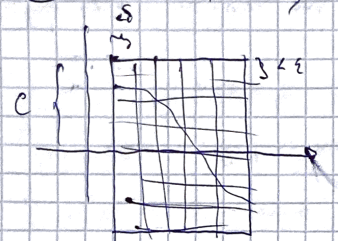
\includegraphics[width=0.4\textwidth]{images/eps-net.png}
        \end{figure}
        Для любой функции $f \in M$ можно выбрать ломаную $\varphi \in L$ такую, что для всех $i \in \{0, \dotsc, n\}$ выполнено $|f(x_i) - \varphi(x_i)| < \varepsilon$. Рассмотрим произвольную точку $x \in [a, b]$ и выберем $i \in \{0, \dotsc, n - 1\}$ такое, что $x \in [x_i, x_{i + 1}]$, тогда:
        \[
            |f(x) - \varphi(x)| \leqslant |f(x) - f(x_i)| + |f(x_i) - \varphi(x_i)| + |\varphi(x) - \varphi(x_i)| <  2\varepsilon + |\varphi(x_{i+1}) - \varphi(x_i)|
        \]

        Первое слагаемое меньше $\varepsilon$ из равностепенной непрерывности, а второе по построению $\varphi$. Оценим слагаемое $|\varphi(x_{i+1}) - \varphi(x_i)|$ отдельно:
        \[|\varphi(x_{i+1}) - \varphi(x_i)| \leqslant |f(x_{i+1}) - \varphi(x_{i+1})| + |f(x_{i+1}) - f(x_i)| + |f(x_i) - \varphi(x_i)| < 3\varepsilon\]

        Таким образом, $\sup\limits_{x \in [a, b]}|f(x) - \varphi(x)| < 5\varepsilon$. Значит, построенное множество $L$ образует конечную $5\varepsilon$-сеть для множества $M$, тогда, в силу произвольности выбора числа $\varepsilon$, множество $M$ вполне ограниченно.\qedhere
    \end{itemize}
\end{proof}